Finalmente, llegados a este punto, se procedío a quantificar hasta que punto es necesario realizar el pulido de ambas superficies transversales de la fibra. Este estudio esta enfocado al hecho que el prototipo Tritium 1, a diferencia del prototipo Tritium 0, únicamente realiza la lectura por una de las dos superficies de cada fibra. El motivo de ello es que, por un lado, se observó la necesidad de imponer una configuración rectilinea en el detector para mejorar su eficiencia de recolección y, en segundo lugar, se tuvieron en cuenta una serie de  equerimientos debidos a seguridad nuclear. 

Debido al hecho de que el prototipo Tritium 1 únicamente mide por un lado y su lado contrario se encuentra totalmente recubierto de teflón, estudiamos la necesidad de pulir ambas caras ya que se trata de un proceso duro y largo. Para ello utilizamos el dispositivo experimental mostrado en la imagen \ref{setupcaras}.

\begin{figure}[hbtp]
\centering
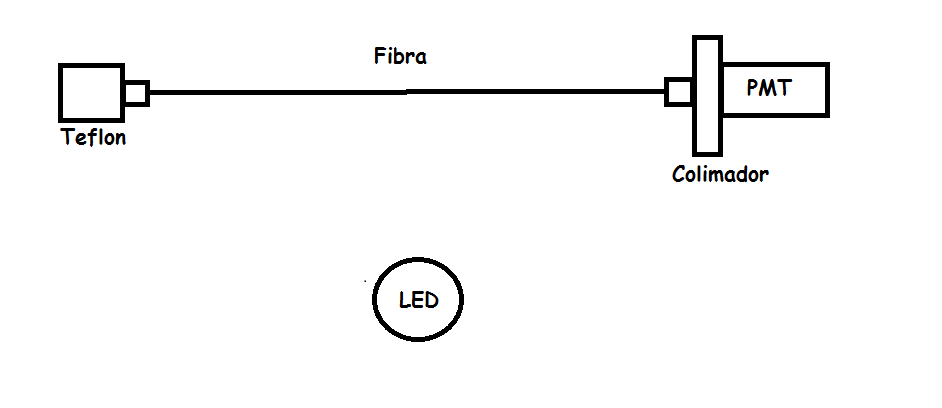
\includegraphics[scale=0.7]{Figuras/SetUpLED.png}
\caption{Dispositivo experimental utilizado para llevar a cabo el estudio.\label{setupcaras}}
\end{figure}

Este consiste en el mismo dispositivo empleado en el estudio anterior pero en el que la LED se ha desplazado a una posición para realizar una incidencia lateral de los fotones. Finalmente, un extremo de la fibra se encuentra totalmente recubierto de teflon y realizamos la lectura de la señal por el otro lado (simulando la situación del detector). Las fibras empleadas fueron de tipo single clad de $200~\mm$ de longitud ya que son las empleadas en el proyecto Tritium.

En primer lugar se realizo este experimento para tres muestras diferentes de fibras en las que solo se había pulido el extremo por el que se realizaba la lectura. En segundo lugar se repitió este mismo experimento con las mismas muestras a las que, además, se les había realizado un segundo pulido en el otro extremo.

Ambos resultados pormediados se muestran en la figura \ref{resultadoscaras}.

\begin{figure}[hbtp]
\centering
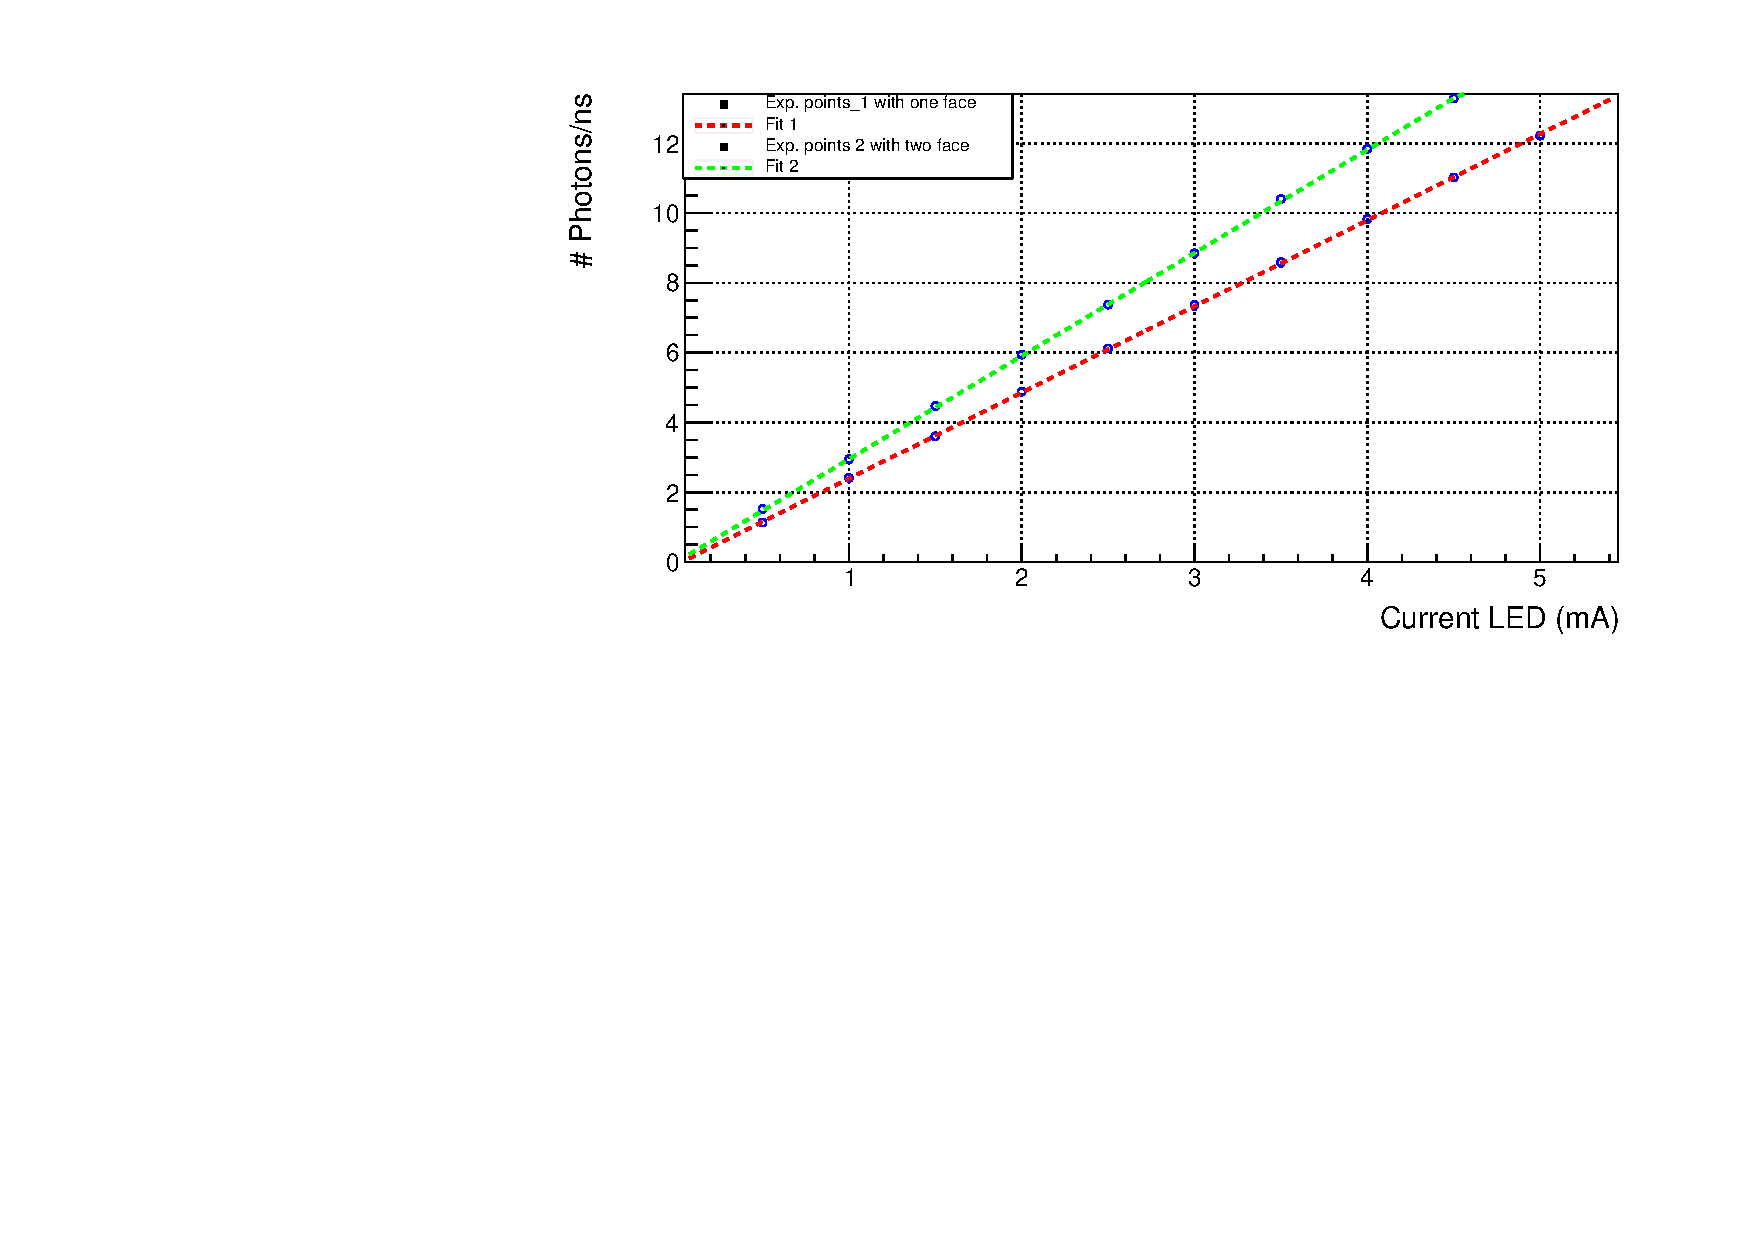
\includegraphics[scale=0.7]{Figuras/casefaces.pdf}
\caption{Intensidad promediada de 3 muestras diferentes de fibras no clad de $200~\mm$ frente a la alimentaicón de la LED con una cara pulida y con ambas.\label{resultadoscaras}}
\end{figure}

Seguidamente, en la figura \ref{diferenciacaras} se presenta la diferencia entre ambas señales:

\begin{figure}[hbtp]
\centering
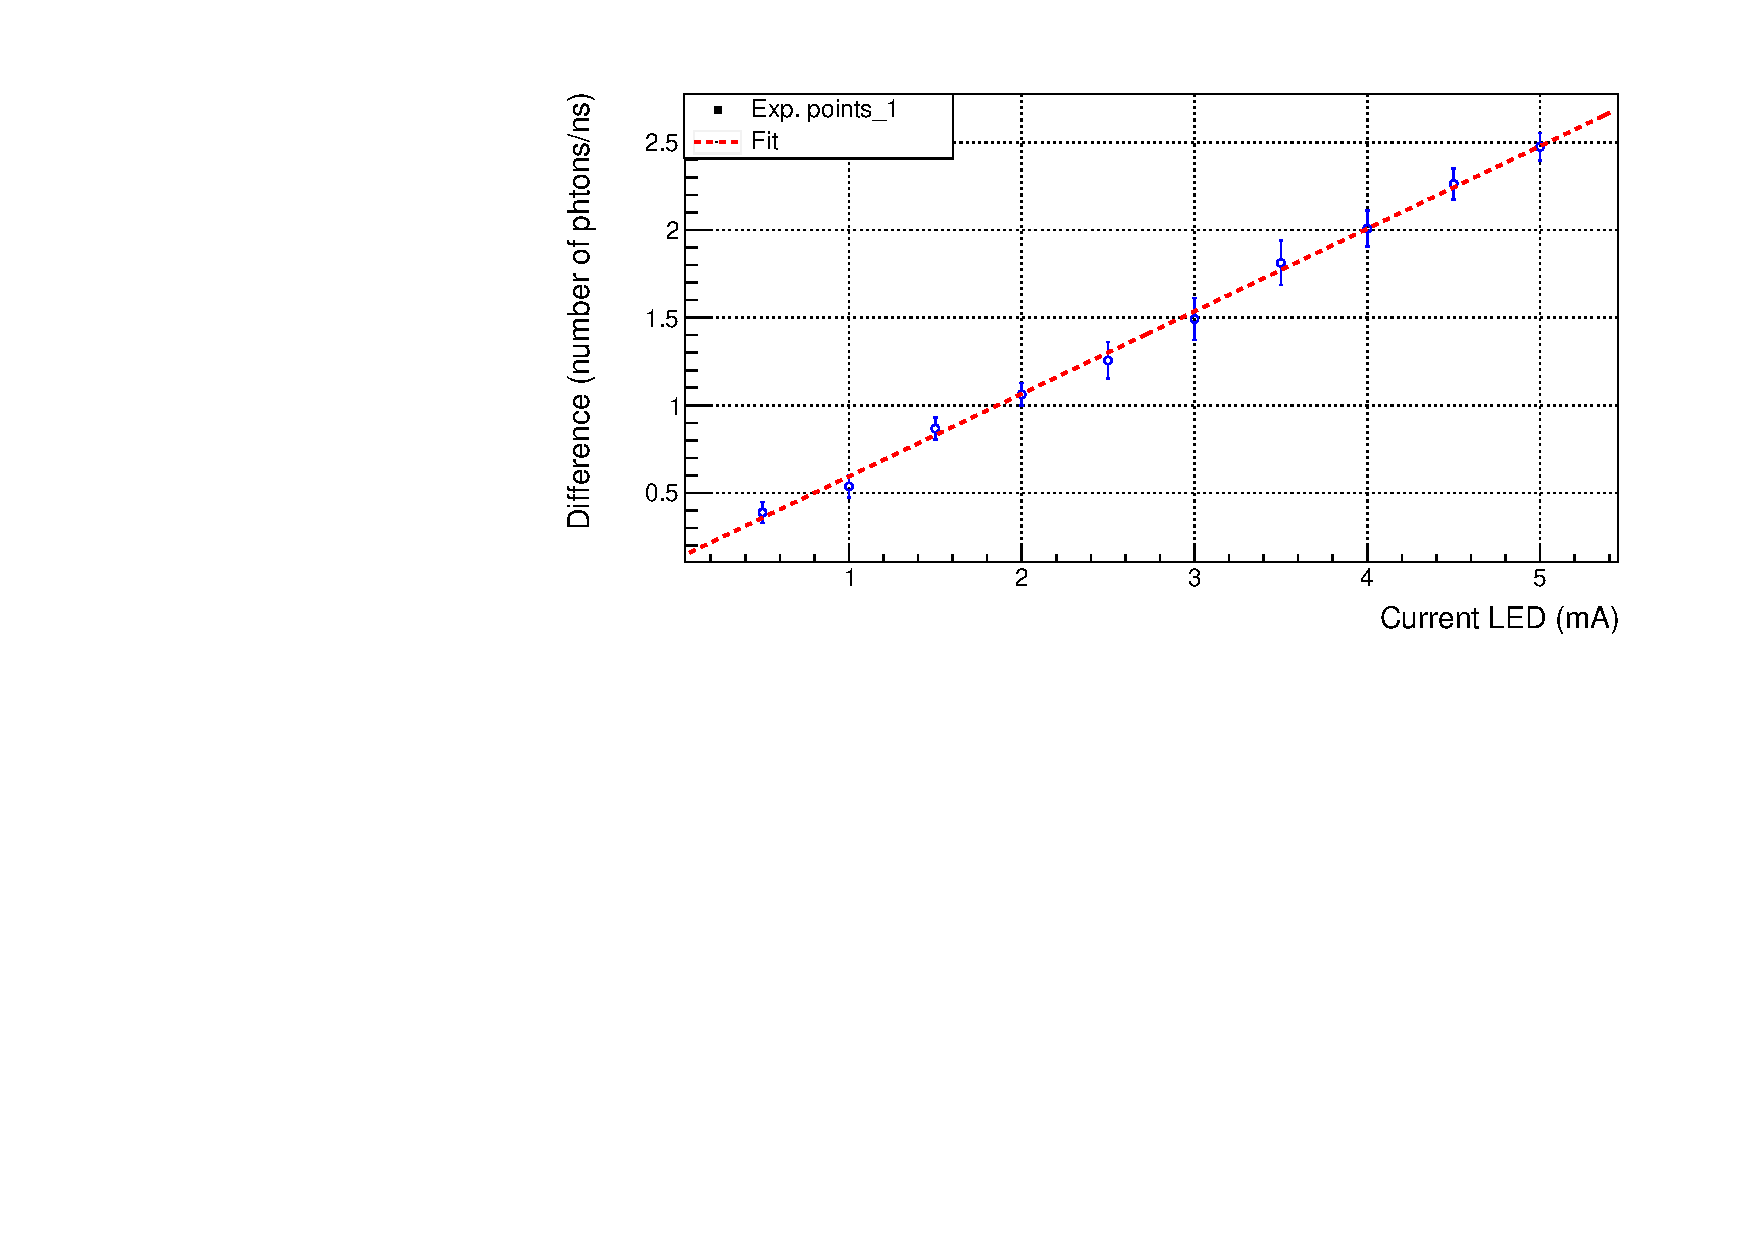
\includegraphics[scale=0.7]{Figuras/Differencefaces.pdf}
\caption{Diferencia entre las señales obtenidas de fibras no clad de $200~\mm$ frente a la alimentaicón de la LED con una cara pulida y con ambas.\label{diferenciacaras}}
\end{figure}

En esta figura podemos observar que, al nivel de señales de aproximadamente 12 fotones por nanosegundo (una tercera parte de las señales debida a eventos del tritio), ya observamos aproximadamente 2.5 fotones por nanosegundo menos en caso de no pulir ambas caras.

Por tanto, al nivel de las señales debidos a los eventos de tritio, si tenemos en cuenta la linealidad observada en el comportamiento, estimamos una perdida de aproximadamente 7.5 fotones por nanosegundo y por fibra. Si utilizamos centenares de fibras o incluso miles tendriamos pérdidas de 750 o 7500 respectivamente. Vemos por tanto que tendríamos una pérdida considerable de fotones, algo que no nos podemos permitir en el proyecto Tritium debido al hecho que ya estamos trabajando con señales excesivamente débiles. Debido a esto, las fibras utilizadas en el prototipo Tritium 1 se pulieron por ambas caras a pesar de realizarse la lectura únicamente por una.

Vemos por tanto que, a pesar de que el extremo se encuentra totalmente recubierto de teflon asegurando de esta manera una reflectividad de los fotones de casi el $100\%$, se necesita ademas un pulido de ambas caras evitando de esta forma una mayor dispersión de los fotones al llegar a este punto. 



